

\section{Model including the second fish}

\begin{flushleft}
    The fishowner desperately wanted two types of competing fish species:
    rainbowfish and gourami. The budget was for 20 rainbowfish and 5 gourami.
    To make sure that both fishes both had enough food and didn't manage to kill eachother
    we made a system of differential equations. In this case they interact with each other.
    There is a 4\% chance that a gourami will kill a rainbowfish, thus the $-0.04PG$.
    Gouramis also don't survive on their own so they slowly die, explaining the $-0.25G$
\end{flushleft}

\begin{align*}[left = \empheqlbrace]
    \frac{dP}{dt}= 0.7P-0.007P^2-0.04PG \\
    \frac{dG}{dt} = -0.25G+0.008PG
\end{align*}

\begin{flushleft}
    Now doing the rest was easy. So easy in fact that I wanted to shoot my foot
    with a rocket launcher. The result was the following:

\end{flushleft}
\begin{center}
    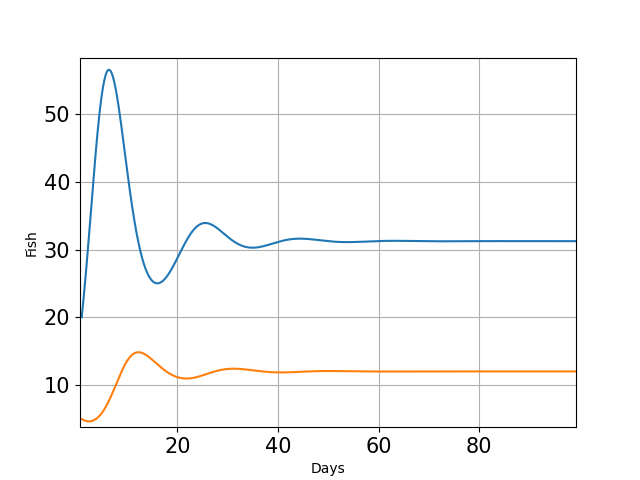
\includegraphics[scale=0.45]{../figures/Figure_2.png}
    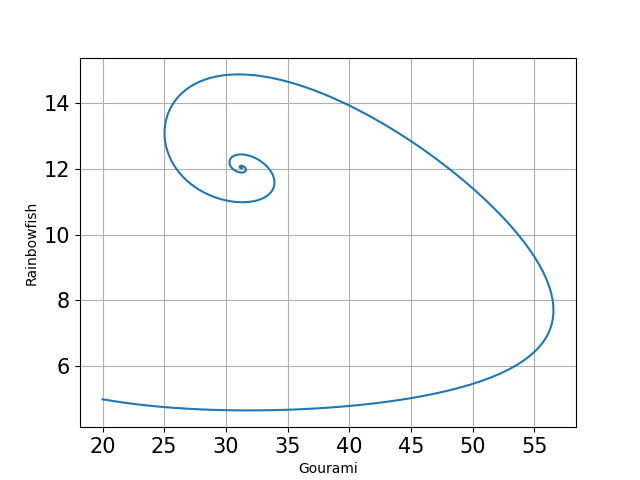
\includegraphics[scale=0.45]{../figures/Figure_3.png}

\end{center}

\begin{flushleft}
    These models tells us that the fish seem to approach an equilibrium at roughtly
    30 rainbowfishes and 12 gourami. The exact equilibrium point is when $\frac{dP}{dt}=0$ and $\frac{dG}{dt}=0$.
    This evaluates to the number of rainbowfish being 31.25 and the amount of gourami is 12.03125. Again, since you
    cannot have fractional fishes the equilibrium is roughly at 31 rainbowfish and 12 gourami.

\end{flushleft}

\begin{flushleft}
    Modelling a few more scenarios with different
    starting populations reveal that there is a stable equilibrium point aslong as
    the amount of fish of one species is more than 0.
\end{flushleft}

\begin{center}
    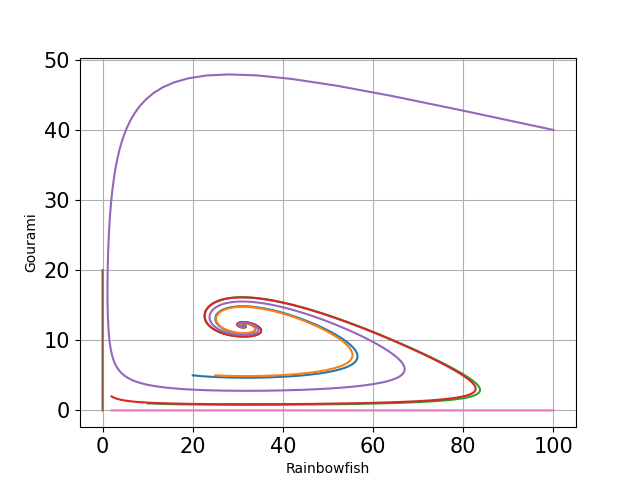
\includegraphics[scale=0.45]{../figures/Figure_4.png}

\end{center}